\documentclass{article}
\title{Getting Started with LLGL}
\author{Lukas Hermanns}
\date{\today}

\usepackage{listings}
\usepackage{color}
\usepackage{pxfonts}
\usepackage{geometry}
\usepackage[T1]{fontenc}
\usepackage{xspace}
\usepackage{hyperref}
\usepackage{graphicx}
\usepackage{float}
\usepackage{pdfpages}

\geometry{
	a4paper,
	left=15mm,
	right=15mm,
	top=20mm,
	bottom=20mm
}

\begin{document}

\definecolor{brightBlueColor}{rgb}{0.5, 0.5, 1.0}
\definecolor{darkBlueColor}{rgb}{0.0, 0.0, 0.5}

\def\LLGL{\textcolor{darkBlueColor}{LLGL}\xspace}

\lstset{
	language = C++,
	basicstyle = \footnotesize\ttfamily,
	commentstyle = \itshape\color{brightBlueColor},
	keywordstyle = \bfseries\color{darkBlueColor},
	stringstyle = \color{red},
	frame = single,
	tabsize = 4,
	showstringspaces=false,
	numbers=none
}

\maketitle


%----------------------------------------------------------------------------------------
%	INTRRODUCTION
%----------------------------------------------------------------------------------------

\begin{figure}[ht]
	\centering
	
\includegraphics[width=0.5\textwidth]{../LLGL_Logo.pdf}
\end{figure}

\section*{Introduction}

\LLGL (Low Level Graphics Library) is a thin abstraction layer for graphics APIs such as
OpenGL, Direct3D, and Vulkan. It is meant to abstract these rendering technologies to one uniform interface.
The library is written entirely in C++11, so you'll
need a modern C++ compiler, i.e. at least \textbf{VisualC++ 2013} for Windows,
\textbf{g++ 4.8} for Linux, or \textbf{Clang 3.1} for MacOS.


%----------------------------------------------------------------------------------------
%	PREREQUISITES
%----------------------------------------------------------------------------------------

\section*{Prerequisites}

To use this library you should be familiar with these subjects:
\begin{itemize}
	\item \textbf{Basic C++11 Programming} \\
	Since the library is written in C++11, you should know something about \emph{smart pointers},
	\emph{raw pointers}, and basic \emph{object-oriented programming} (OOP) in C++.
	
	\item \textbf{Basic Linear Algebra} \\
	You should be familiar with at least \emph{Vectors} and \emph{Matrices}.
	
	\item \textbf{Fundamentals in Graphics Programming} \\
	You should be familiar with the fundamentals of graphics programming, since this is only a low-level graphics library.
	You should also be familiar with at least one of the major graphics APIs,
	i.e. \emph{OpenGL}, \emph{Direct3D}, \emph{Vulkan}, \emph{Mantle}, or \emph{Metal},
	because \LLGL does only little to no higher abstractions.
	
	\item \textbf{Shading Languages} \\
	\LLGL forces you to always write your own shaders, so you should be familiar with
	\href{https://www.opengl.org/documentation/glsl/}{GLSL} or
	\href{https://msdn.microsoft.com/de-de/library/windows/desktop/bb509561(v=vs.85).aspx}{HLSL}.
\end{itemize}


%----------------------------------------------------------------------------------------
%	PROGRESS
%----------------------------------------------------------------------------------------

\newpage
\section*{Progress}

This project is still in its early steps. Here is a short overview of its progress:

\subsection*{Platforms}
\begin{itemize}
	\item \textbf{Windows} \\
	Windows 10 is the main development environment of the author, so this platform has the best support.
	
	\item \textbf{MacOS} \\
	The MacOS port is in its early steps, but a few tutorials are already running.
	The development environment for the MacOS port is \emph{macOS Sierra}.
	
	\item \textbf{Linux} \\
	Kubuntu 16 (GNU/Linux) is used inside a virtual machine by the author to develop the linux port.
	This platform is partially supported (i.e. anti-aliasing or other features are not complete on this platform).
\end{itemize}
	
\subsection*{Renderers}
\begin{itemize}
	\item \textbf{OpenGL} \\
	OpenGL renderer is almost done (\textasciitilde 85\% complete).
	
	\item \textbf{Direct3D 11} \\
	Direct3D 11 renderer is almost done (\textasciitilde 85\% complete).
	
	\item \textbf{Direct3D 12} \\
	Direct3D 12 renderer is only in an experimental state (\textasciitilde 5\% complete).
	
	\item \textbf{Vulkan} \\
	Vulkan renderer is scheduled, but not supported yet.
\end{itemize}


%----------------------------------------------------------------------------------------
%	BUILD PROCESS
%----------------------------------------------------------------------------------------

\newpage
\section*{Build Process}

\subsection*{Dependencies}

\subsubsection*{GaussianLib}

The only required dependency is the header-only library
\href{https://github.com/LukasBanana/GaussianLib}{\textsc{GaussianLib}},
which is used for basic linear algebra computations with vectors and matrices.

\subsubsection*{OpenGL}

To build the OpenGL render system you need the OpenGL extension header files and an up-to-date graphics driver.
For Windows the header files \texttt{glext.h} and \texttt{wglext.h} are required.
For Linux the header files \texttt{glext.h} and \texttt{glxext.h} are required.
For MacOS no header files need to be downloaded, since the OpenGL version depends on the OS version.
You can find the header files at the \href{https://www.opengl.org/registry/#headers}{OpenGL registry page}.
Place the header files in the \texttt{include/GL/} folder of your compiler environment
or add the include path later in your build settings.

\subsubsection*{Direct3D}

Since VisualStudio 2013, the DirectX framework (of which Direct3D is a part of) is included within
the VisualStudio setup, so no further SDK needs to be installed.

%\subsubsection*{Vulkan}

%To build the Vulkan render system you need the \href{https://lunarg.com/vulkan-sdk/}{Vulkan SDK},
%and of course a graphics driver which supports at least Vulkan 1.0.

\subsection*{Build Tool}

To build the \LLGL project files you need the build tool \href{https://cmake.org/}{CMake 2.8} or later.
The build process is now demonstrated with the CMake GUI on Windows, but it can also be configured
on a command line (more about this see \href{https://cmake.org/runningcmake/}{cmake.org/runningcmake}).

Set the source directory (``Where is the source code:'') to the \LLGL repository
and set the build directory (``Where to build the binaries'') where you want your project files.
In this example (see \ref{fig:cmake_mask1}) the source directory is \texttt{<\dots>/LLGL/repository}
and the build directory is \texttt{<\dots>/LLGL/build\_msvc14} because the project files are build
for MSVC14 (VisualStudio 2015).

Now set the \textsc{GaussianLib} include directory (in this example \texttt{<...>/GaussianLib/repository/include})
and click on ``Configure''. If everything worked quite well, you should see the message ``Configuring done''
in the lower box. To finally create the project files, clock on ``Generate''.
Then your project files should be located in the build directory you just set up previously.

\begin{figure}[H]
	\centering
	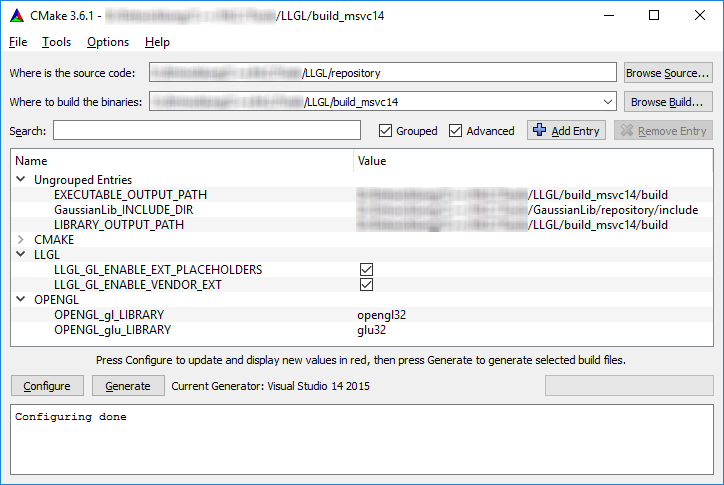
\includegraphics[width=0.9 \textwidth]{cmake_mask1}
	\caption{CMake GUI mask to set up the project files for VisualStudio 2015 (MSVC14).}
	\label{fig:cmake_mask1}
\end{figure}

There are a few options you can switch on and off, which will enable or disable the respective macro
when you compile the project:
\begin{itemize}
	\item \texttt{LLGL\_BUILD\_(TESTS/TUTORIALS/RENDERER\_\dots)} \\
	Specifies whether to include all test, all tutorials, or the repsective renderer projects.
	
	\item \texttt{LLGL\_ENABLE\_CHECKED\_CAST} \\
	Specifies whether to enable or disable dynamic checked casts.
	This is only available in debug mode.
	
	\item \texttt{LLGL\_ENABLE\_DEBUG\_LAYER} \\
	Specifies whether to enable or disable the debug layer.
	This is a wrapper around the render system and all other render objects for effective debugging.
	
	\item \texttt{LLGL\_ENABLE\_UTILITY} \\
	Specifies whether to enable or disable utility functions, which can be used to easily initialize descriptor structures.
	They must be included separately with the \texttt{LLGL/Utility.h} header file.
	
	\item \texttt{LLGL\_GL\_ENABLE\_EXT\_PLACEHOLDERS} \\
	Specifies whether OpenGL extensions should be replaced by placeholder procedures
	when they are not available. This may help debugging and should not influence the runtime performance.
	
	\item \texttt{LLGL\_GL\_ENABLE\_VENDOR\_EXT} \\
	Specifies whether vendor specific OpenGL extensions should be enabled or disabled.
	One of these extensions is for conservative rasterization
	(\texttt{GL\_NV\_conservative\_raster} and \texttt{GL\_INTEL\_conservative\_rasterization}) for instance.
	These extensions will only be loaded and used by the runtime if they are available on the host platform.
\end{itemize}


%----------------------------------------------------------------------------------------
%	API OVERVIEW
%----------------------------------------------------------------------------------------

\newpage

\section*{API Overview}

LLGL has a very simple and unified API design.
For object creation, there is commonly a ``\texttt{\dots Descriptor}'' structure (e.g. \texttt{LLGL::ImageDescriptor}),
which contains all necessary information to describe the object which is to be created.
There are three major interfaces: \emph{RenderSystem} is mainly used for object creation and memory read/write operations,
\emph{RenderContext} is used to configure each framebuffer and its back buffer (or rather swap chain),
and \emph{CommandBuffer} which is used to set render states, draw primitives, and dispatch compute commands.

\subsection*{RenderSystem}

In the RenderSystem interface there are several functions of the following form:
\begin{lstlisting}
// Create a new object
Create...

// Update the data of an object
Write...

// Read the data from an object
Read...

// Map the memory of an object from GPU to CPU memory space
Map...

// Unmap the memory from an object
Unmap...

// Release the object
Release
\end{lstlisting}

\subsection*{CommandBuffer}

There are several overloaded functions for drawing operations with the naming convention
``\texttt{Draw}'', ``\texttt{DrawIndexed}'', ``\texttt{DrawInstanced}'', or ``\texttt{DrawIndexedInstanced}''.
The most other functions are used to configure the command buffer of the graphics API, which have the following form:
\begin{lstlisting}
// Set a hardware buffer/ texture/ sampler etc.
Set...

// Begin and always end a state (e.g. BeginQuery/ EndQuery)
Begin...
End...

// Draw primitives
Draw...
\end{lstlisting}


%----------------------------------------------------------------------------------------
%	HELLO TRIANGLE
%----------------------------------------------------------------------------------------

\newpage

\section*{Hello Triangle}

After we have set up and build the library, we can start rendering some geometry.
Our example will consist of a single C++ source file (e.g. ``\texttt{main.cpp}'') and two shader files
(e.g. ``\texttt{vertex.glsl}'' and ``\texttt{fragment.glsl}'').
The include path for a project, that uses \LLGL, must be set to \texttt{\textit{<your-LLGL-repository>}/include/},
and the \LLGL library file must be added to the linker (for Windows this is ``\texttt{LLGL.lib}''
when compiling in Release mode and ``\texttt{LLGLD.lib}'' when compiling in Debug mode).
All the other library files don't need to be added to the linker (e.g. ``\texttt{LLGL\_OpenGL.lib}''),
since the respective renderer module is loaded at runtime.

Now let's start with a small example. At first we need to include the header files.
The main header we need is \texttt{LLGL/LLGL.h} where the entire \LLGL interface is declared.
For our example we also need basic I/O classes from \texttt{iostream} for standard output, \texttt{fstream}
to read the shader files, and \texttt{Gauss/Gauss.h} for some matrix classes:
\begin{lstlisting}
#include <LLGL/LLGL.h>
#include <Gauss/Gauss.h>
#include <iostream>
#include <fstream>
\end{lstlisting}
Next we define the C++ main function and wrap the entire example code into a large \texttt{try-catch} block,
to quit the application with a meaningful error message if any failure happens:
\begin{lstlisting}
int main() {
    try {
        /* example code here ... */
    } catch (const std::exception& e) {
        std::cerr << e.what() << std::endl;
    }
    return 0;
}
\end{lstlisting}
To create an \LLGL renderer instance in our main function, we load a renderer module
(a \textit{module} here denotes a dynamic shared library)
from the static \texttt{Load} function of the \texttt{RenderSystem} interface:
\begin{lstlisting}
std::shared_ptr<LLGL::RenderSystem> renderer = LLGL::RenderSystem::Load("OpenGL");
\end{lstlisting}
Here we could actually use the C++11 keyword \texttt{auto} to simplify the code,
but for explanation purposes we keep the types explicit.
Most creation or load functions return a new instance wrapped in a \texttt{std::unique\_ptr},
but in this case \LLGL needs to keep track of the instance to check if it has already been expired,
which is only feasible with an \texttt{std::shared\_ptr}.

Moreover, most functions use enumerations instead of strings to specify some type, but in this case
a module can be loaded dynamically at runtime and further modules can be added or removed independently.
Therefore the renderer module is specified by a string (here ``OpenGL''). Other modules are
named ``Direct3D11'', ``Direct3D12'', and ``Vulkan''.
Whenver you load a new renderer, there must not remain any references to this shared object,
because only a single renderer can be loaded at a time.
When this shared object expires, all objects allocated by this renderer will be deleted automatically.

If loading the renderer failed, an \texttt{std::runtime\_error} exception will be thrown,
which can be cached to show an error message and/or load another renderer module instead.
This can be very handy if a specific Direct3D version is not installed on the host Windows platform,
so another Direct3D version or OpenGL renderer can be loaded as fallback
without disturbing the user with akward error messages and program crashes.

After we created the renderer we need a graphics context to draw into.
This is done by the \texttt{CreateRenderContext} function which takes a descriptor structure:
\begin{lstlisting}
LLGL::RenderContextDescriptor contextDesc;
{
    contextDesc.videoMode.resolution = { 640, 480 };
}
LLGL::RenderContext* context = renderer->CreateRenderContext(contextDesc);
\end{lstlisting}
This is a minimal example for the render context descriptor. There are much more attributes
to specify multi-sampled anti-aliasing, vertical-synchronisation, etc.
See the API documentation for more information about these attributes.

This render context will create its own window, but we could also specifiy our own one.
However, in this example we keep it simple. To access this window and change the title,
we use the \texttt{GetWindow} function of the \texttt{RenderContext} interface
which returns a reference to its window:
\begin{lstlisting}
context->GetWindow().SetTitle(L"LLGL Tutorial 01: Hello Triangle");
\end{lstlisting}
Since some platforms (such as Win32) support Unicode window titles, our string literal starts with the `L' token.

\newpage
\noindent
Next we create a vertex buffer to store our geometry. For this example we give up an index buffer,
since we only draw a single triangle and no complex models. At first we define our vertex data and the vertex format,
which is required to tell the rendering API how the vertex attributes are located within the vertex buffer:
\begin{lstlisting}
// Vertex data structure
struct Vertex {
    Gs::Vector2f    position;
    LLGL::ColorRGBf color;
};

// Vertex data (3 vertices for our triangle)
Vertex vertices[] = {
    { {  0,  1 }, { 1, 0, 0 } }, // 1st vertex: center-top, red
    { {  1, -1 }, { 0, 1, 0 } }, // 2nd vertex: right-bottom, green
    { { -1, -1 }, { 0, 0, 1 } }, // 3rd vertex: left-bottom, blue
};

// Vertex format
LLGL::VertexFormat vertexFormat;
vertexFormat.AppendAttribute({ "position", LLGL::VectorType::Float2 }); // position has 2D float vector
vertexFormat.AppendAttribute({ "color",    LLGL::VectorType::Float3 }); // color has 3D float vector
\end{lstlisting}
The \texttt{AppendAttribute} function adds the attributes to the vertex format.
The order of these function calls determines the location in the vertex data, so they must match
the order of the member fields in the vertex data structure (here ``\texttt{struct Vertex}'').

Now we can create our vertex buffer and upload the vertex data to the GPU by passing a pointer
to the \texttt{initialData} parameter:
\begin{lstlisting}
LLGL::BufferDescriptor bufferDesc;

// Set the common buffer attributes
bufferDesc.type = LLGL::BufferType::Vertex; // Buffer type
bufferDesc.size = sizeof(vertices);         // Size (in bytes) of the buffer

// Set vertex buffer specific attributes
bufferDesc.vertexBuffer.format = vertexFormat; // Copy the vertex format

LLGL::Buffer* vertexBuffer = renderer->CreateBuffer(bufferDesc, vertices);
\end{lstlisting}
To update an entire hardware buffer or texture (or only a portion of it) there is a respective
``\texttt{Write...}'' function.

Now we have the vertex buffer complete and we can cross over to shader creation.
In \LLGL the shaders (Vertex, Tessellation-Control, Tessellation-Evaluation, Geometry, Fragment, and Compute shaders)
are created independently, and then attached and linked together with a shader program.
For our example we only need a Vertex- and Fragment (also called ``Pixel'') shader:
\begin{lstlisting}
LLGL::Shader* vertexShader = renderer->CreateShader(LLGL::ShaderType::Vertex);
LLGL::Shader* fragmentShader = renderer->CreateShader(LLGL::ShaderType::Fragment);
\end{lstlisting}
Now we have two empty shaders. Next we load the shader code from file with
our custom ``\texttt{ReadFileContent}'' lambda function:
\begin{lstlisting}
// Define the lambda function to read an entire text file
auto ReadFileContent = [](const std::string& filename) {
    std::ifstream file(filename);
    return std::string( ( std::istreambuf_iterator<char>(file) ),
                        ( std::istreambuf_iterator<char>(    ) ) );
};

// Load vertex- and fragment shader code from file
std::string vertexShaderCode = ReadFileContent("vertex.glsl");
std::string fragmentShaderCode = ReadFileContent("fragment.glsl");
\end{lstlisting}

\newpage
\noindent
After reading the shader code into strings we can compile the shaders:
\begin{lstlisting}
auto CompileShader = [](LLGL::Shader* shader, const std::string& code) {
    // Compile shader
    shader->Compile(code);
    
    // Print info log (warnings and errors)
    std::string log = shader->QueryInfoLog();
    if (!log.empty()) {
        std::cerr << log << std::endl;
    }
};

CompileShader(vertexShader, vertexShaderCode);
CompileShader(fragmentShader, fragmentShaderCode);
\end{lstlisting}
Shader compilation works a little different between GLSL (for OpenGL) and HLSL (for Direct3D).
For HLSL shader compilation there is a second overloaded ``\texttt{Compile}'' function with more parameters,
to specifiy the entry point and shader version target.

Having the shaders compiled, we can now create a shader program, attach all shaders to it,
bind the vertex attribute layout, and finally link the shader program:
\begin{lstlisting}
// Create shader program which is used as composite
LLGL::ShaderProgram* shaderProgram = renderer->CreateShaderProgram();

// Attach vertex- and fragment shader to the shader program
shaderProgram->AttachShader(*vertexShader);
shaderProgram->AttachShader(*fragmentShader);

// Build vertex layout for input assembly (this is not required for a compute shader program)
shaderProgram->BuildInputLayout(vertexFormat);

// Link shader program and check for errors
if (!shaderProgram->LinkShaders()) {
    throw std::runtime_error(shaderProgram->QueryInfoLog());
}
\end{lstlisting}
The ``\texttt{BuildInputLayout}'' function binds the vertex attributes to the shader program.
This must be called after shader attachment but before shader linking (except a compute shader program is used).

Before we continue with the C++ code, we first take a look at the shader code:
\begin{lstlisting}[title={\texttt{vertex.glsl}}]
// GLSL shader version 1.30 (for OpenGL 3.1)
#version 130

// Vertex attributes (these names must match our vertex format attributes)
in vec2 position;
in vec3 color;

// Vertex output to the fragment shader
out vec3 vertexColor;

// Vertex shader main function
void main() {
    gl_Position = vec4(position, 0, 1);
    vertexColor = color;
}
\end{lstlisting}
This simple vertex shader only passes the vertex position and color (with default interpolation) to the fragment shader.

\newpage
\noindent
And here is the fragment shader:
\begin{lstlisting}[title={\texttt{fragment.glsl}}]
// GLSL shader version 1.30 (for OpenGL 3.1)
#version 130

// Fragment input from the vertex shader
in vec3 vertexColor;

// Fragment output color
out vec4 fragColor;

// Fragment shader main function
void main() {
    fragColor = vec4(vertexColor, 1);
}
\end{lstlisting}

Now we are finally done with setting up the shader. Next we need to create a graphics pipeline.
This concept is derived from modern graphics APIs such as Direct3D 12 and Vulkan.
The major pipeline state is stored inside this pipeline state object.
For older graphics APIs (such as OpenGL) \LLGL will set the respective render states by its internal state manager,
to reduce state changes.

The graphics pipeline specifies the depth-, stencil-, rasterizer-, blending-,
and shader states and is created as follows:
\begin{lstlisting}
LLGL::GraphicsPipelineDescriptor pipelineDesc;
{
    pipelineDesc.shaderProgram = shaderProgram;
}
LLGL::GraphicsPipeline* pipeline = renderer->CreateGraphicsPipeline(pipelineDesc);
\end{lstlisting}
In our example we can use all default settings of the graphics pipeline descriptor except the shader program,
which must always be set by the client programmer.

Before we start with the render main loop, we need a command buffer which can send render state and draw commands to the GPU:
\begin{lstlisting}
// Create command buffer to submit subsequent graphics commands to the GPU
LLGL::CommandBuffer* commands = renderer->CreateCommandBuffer();

// Set the render context as the initial render target
commands->SetRenderTarget(*context);
\end{lstlisting}
We now have all render objects, so we can start with the main loop:
\begin{lstlisting}
// Run main loop until the main window is closed
while (context->GetWindow().ProcessEvents()) {
    /* render code here ... */
}
\end{lstlisting}
This main loop will run until the user clicks the close button on the window of the render context.
The rest of the code is pretty simple, since the most work is done during initialization.
What we need to do is to clear the color buffer of the previous frame,
set the graphics pipeline, set the vertex buffer, draw the primitives, and present the result on the frame buffer:
\begin{lstlisting}
// Set viewport (left: 0, top: 0, width: 640, height: 480)
commands->SetViewport({ 0, 0, 640, 480 });

// Clear color buffer
commands->Clear(LLGL::ClearFlags::Color);

// Bind graphics pipeline
commands->SetGraphicsPipeline(*pipeline);

// Bind vertex buffer
commands->SetVertexBuffer(*vertexBuffer);

// Generate 3 vertices to draw a triangle
commands->Draw(3, 0);

// Present the result on the frame buffer (or rather on the screen)
context->Present();
\end{lstlisting}
When you have done everything right, you should see something like shown in figure \ref{fig:tut01_mask1} after compilation
and program start.
\begin{figure}[H]
	\centering
	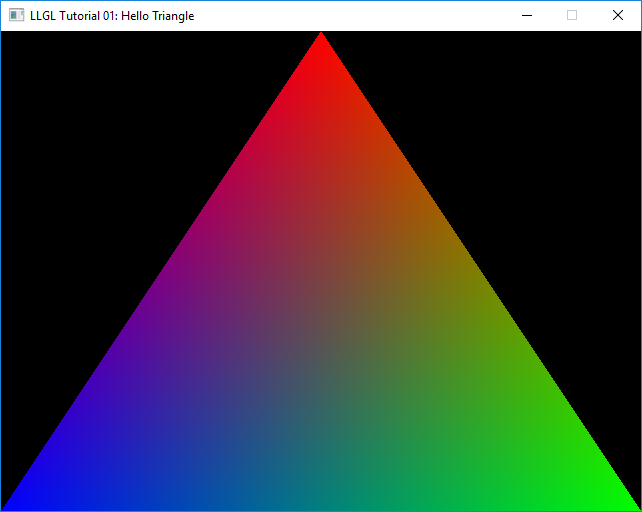
\includegraphics[width=0.8 \textwidth]{tut01_mask1a}
	\caption{Output of the ``Tutorial01: HelloTriangle'' running on Windows 10.}
	\label{fig:tut01_mask1}
\end{figure}




%----------------------------------------------------------------------------------------
%	APPENDIX
%----------------------------------------------------------------------------------------

%\newpage

%\section*{Appendix}

%Foo bar ...






\end{document}
